\section{Atomic Structure of Alkali-Metal Memories}
\label{sec}

Alkali-metal atoms are well suited to ensemble quantum memories because their single valence electron produces a comparatively simple spectrum of electronic, hyperfine, and Zeeman states. The optically allowed $D_1$ and $D_2$ transitions provide strong coupling to the signal and control fields, while the hyperfine-split ground states support coherences with lifetimes far exceeding that of the optical excited state~\cite{Qmeaara_HeshamiEtAl_2016,JiangEtAl_2016,Apgteitiav_FinkelsteinEtAl_2023}. This combination naturally provides the two long-lived lower states and the optically accessible excited state required for a $\Lambda$-type memory. Rubidium (Rb) and Cessium (Cs) are therefore considered in the simulations presented in this work. Although they differ in atomic mass, transition wavelength, hyperfine splitting, and operating conditions, both can be prepared as warm vapours or laser-cooled ensembles and described within the same restricted level structure relevant to optical storage~\cite{Oqmboeit_MaEtAl_2017}.

Alkali atoms are widely used in quantum optics because their strongest optical transitions lie in the near-infrared spectral region. Narrow-linewidth diode lasers, modulators, detectors, and standard optical components are readily available at these wavelengths. These technical features are particularly important for quantum memories protocols because the signal and control fields must address selected transitions, maintain stable frequency detunings, and allow the weak retrieved field to be separated from the strong classical control field \cite{Oqmboeit_MaEtAl_2017}.

\textbf{Relevant Lines} 
The optical transitions relevant to alkali-metal memories are the $D_1$ and $D_2$ lines, corresponding respectively to $n^2S_{1/2}\rightarrow n^2P_{1/2}$ and $n^2S_{1/2}\rightarrow n^2P_{3/2}$~\cite{CsDataLineSteck,RbDataLineSteck}. The present work considers the $D_1$ line, located near \SI{894.6}{\nano\metre} for the $6^2S_{1/2}\rightarrow6^2P_{1/2}$ transition in ${}^{133}\mathrm{Cs}$ and near \SI{795}{\nano\metre} for the $5^2S_{1/2}\rightarrow5^2P_{1/2}$ transition in ${}^{87}\mathrm{Rb}$~\cite{CsDataLineSteck,RbDataLineSteck,Oqmboeit_MaEtAl_2017}.

The optically excited state is unsuitable for long-lived storage because the associated population and optical coherence decay through spontaneous emission and optical dephasing. The storage states are instead selected from the hyperfine levels of the electronic ground state. Hyperfine structure arises from the coupling of the nuclear angular momentum $\hat{\mathbf I}$ to the electronic angular momentum $\hat{\mathbf J}$. The resulting total angular momentum is~\cite{CsDataLineSteck,RbDataLineSteck}
$\hat{\mathbf F}
=
\hat{\mathbf I}
+
\hat{\mathbf J} 
$ with the eigenstates $\ket{F,m_F}$ that satisfy:
\begin{equation}
\hat{F}^{2}\ket{F,m_F}
=
\hbar^{2}F(F+1)\ket{F,m_F},
\qquad
\hat{F}_{z}\ket{F,m_F}
=
\hbar m_F\ket{F,m_F},
\label{eq:hyperfine_angular_momentum}
\end{equation}
where $F$ is the hyperfine angular-momentum quantum number and $m_F$ is its projection along the quantization axis.

For ${}^{133}\mathrm{Cs}$, the $6^2S_{1/2}$ ground state is divided into the $F=3$ and $F=4$ hyperfine manifolds, separated by approximately \SI{9.193}{\giga\hertz}~\cite{CsDataLineSteck}. The two storage states may therefore be selected as
\begin{equation}
\ket{g}
=
\ket{6^2S_{1/2},F=3,m_g},
\qquad
\ket{s}
=
\ket{6^2S_{1/2},F=4,m_s},
\label{eq:cs_memory_states}
\end{equation}
where $m_g$ and $m_s$ denote the selected Zeeman sublevels.

For ${}^{87}\mathrm{Rb}$, the $5^2S_{1/2}$ ground state is divided into the $F=1$ and $F=2$ manifolds, separated by approximately \SI{6.835}{\giga\hertz}~\cite{RbDataLineSteck}. The corresponding storage states may be written as
\begin{equation}
\ket{g}
=
\ket{5^2S_{1/2},F=1,m_g},
\qquad
\ket{s}
=
\ket{5^2S_{1/2},F=2,m_s}.
\label{eq:rb_memory_states}
\end{equation}
In both species, the selected ground-state pair supports a coherence whose lifetime is substantially longer than that of the optical excited state. The values of $m_g$ and $m_s$ are determined by the optical polarizations, selection rules, and magnetic-field configuration used to define the effective memory transition.

Figure~\ref{fig} shows the complete hyperfine structure of the $D_1$ lines from which the effective memory levels are selected. In each species, the two ground-state hyperfine manifolds provide the long-lived storage states, while the excited-state hyperfine manifolds provide the optical transitions addressed by the signal and control fields.

The excited state $\ket{e}$ is selected from the corresponding $D_1$ excited manifold. For Cs it belongs to $6^2P_{1/2}$, while for Rb it belongs to $5^2P_{1/2}$. More completely, the selected state may be denoted by $\ket{e}=\ket{n^2P_{1/2},F',m_e}$, where the excited hyperfine quantum number $F'$ and Zeeman sublevel $m_e$ depend on the addressed transition. The signal field couples $\ket{g}$ to $\ket{e}$, while the control field couples $\ket{s}$ to the same excited state,
\begin{equation}
\ket{g}
\leftrightarrow
\ket{e},
\qquad
\ket{s}
\leftrightarrow
\ket{e}.
\label{eq:lambda_transitions}
\end{equation}
The two optical couplings therefore establish a $\Lambda$ system in which the signal and control fields create a coherence between the long-lived states $\ket{g}$ and $\ket{s}$~\cite{Apgteitiav_FinkelsteinEtAl_2023,Oqmboeit_MaEtAl_2017}.

The allowed couplings are determined by the electric-dipole selection rules. At the hyperfine level, the transitions satisfy~\cite{CsDataLineSteck,RbDataLineSteck}
\begin{equation}
\Delta F
=
0,\pm1,
\qquad
F=0
\not\rightarrow
F'=0,
\label{eq:selection_rule_F}
\end{equation}
together with
\begin{equation}
\Delta m_F
=
0,\pm1.
\label{eq:selection_rule_mF}
\end{equation}
The change in $m_F$ is fixed by the optical polarization. A $\pi$-polarized field drives $\Delta m_F=0$, while $\sigma^{+}$ ($\sigma^{-}$) polarizations drive $\Delta m_F=+1\, (-1)$, respectively~\cite{CsDataLineSteck,RbDataLineSteck,Apgteitiav_FinkelsteinEtAl_2023}.

The $\Lambda$ model retains one pair of ground-state hyperfine--Zeeman levels and one common excited state from the full Cs or Rb level structure. All remaining hyperfine and Zeeman states are excluded. This reduction is appropriate when the signal and control frequencies and polarizations predominantly address the selected transitions, while coupling to neighbouring levels is sufficiently off resonant. The retrieval model developed in sec.~\ref{sec:Model} does not solve the full internal-state dynamics. Instead, the stored ground-state coherence is introduced directly as a spin-wave amplitude, and the atomic species enters through the $D_1$ wavelength, atomic mass, motional parameters, and differential Zeeman response. The ground-state splitting fixes the signal--control frequency difference required for two-photon resonance. Optical pumping, multilevel light shifts, and noise generated by off-resonant transitions are therefore outside the scope of the model.

% The [H] placement specifier requires \usepackage{float} in the main preamble.
\begin{figure}[tbp]
    \centering
    \begin{minipage}[t]{0.495\textwidth}
        \centering
        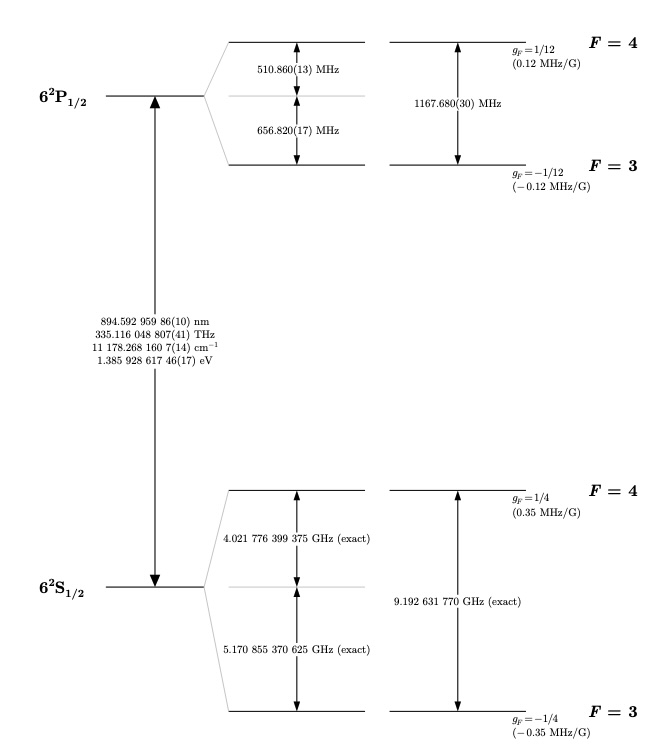
\includegraphics[width=\linewidth]{Figures/cs133_d1_hyperfine.jpeg}
        \par\smallskip
        \textbf{(a)} \({}^{133}\mathrm{Cs}\) D$_1$ line.
    \end{minipage}\hfill
    \begin{minipage}[t]{0.495\textwidth}
        \centering
        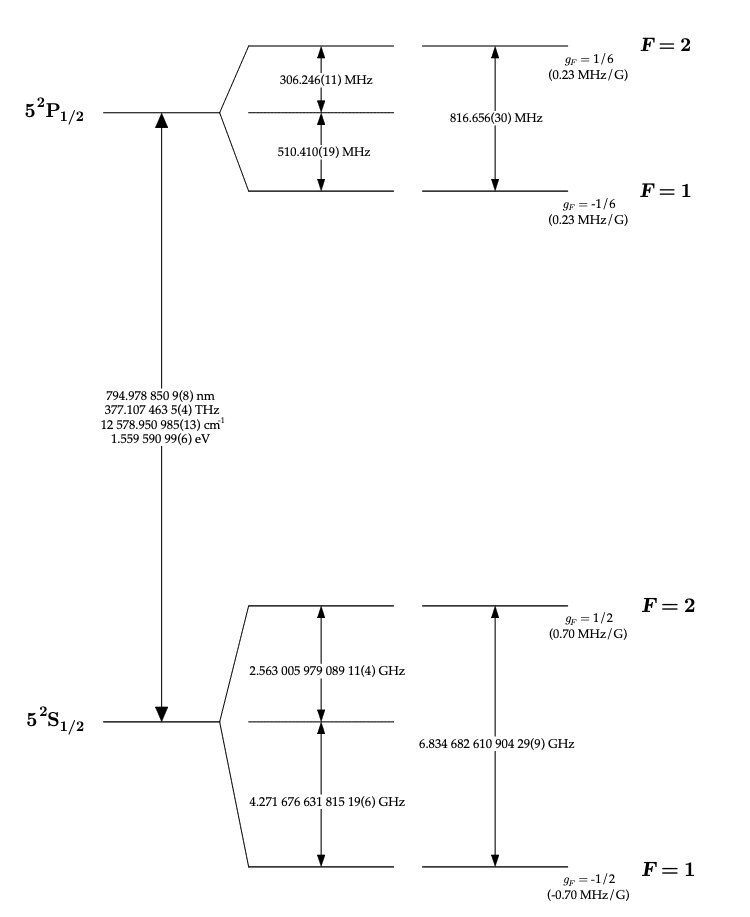
\includegraphics[width=\linewidth]{Figures/rb87_d1_hyperfine.jpeg}
        \par\smallskip
        \textbf{(b)} \({}^{87}\mathrm{Rb}\) D$_1$ line.
    \end{minipage}
    \caption[Hyperfine structure of the Cs and Rb D$_1$ lines.]{
        Hyperfine structure of the D$_1$ transitions used to construct alkali-metal
        \(\Lambda\)-type memories: \textbf{(a)} the
        \(6^2S_{1/2}\rightarrow6^2P_{1/2}\) transition of
        \({}^{133}\mathrm{Cs}\), reproduced from Ref.~\cite{CsDataLineSteck}, and
        \textbf{(b)} the \(5^2S_{1/2}\rightarrow5^2P_{1/2}\) transition of
        \({}^{87}\mathrm{Rb}\), reproduced from Ref.~\cite{RbDataLineSteck}.
        The diagrams show the ground- and excited-state hyperfine splittings and
        the approximate Land\'e factors. Splittings are drawn to scale within each
        hyperfine manifold, but the optical separation and the relative spacing
        of different manifolds are not shown on a common scale.
    }
    \label{fig:cs_rb_d1_hyperfine}
\end{figure}
